\documentclass[12pt]{book}

\usepackage{amsthm}
\usepackage{amsmath}
\usepackage{amsfonts}
\usepackage{mathrsfs}
\usepackage{array}
\usepackage{amssymb}
\usepackage{units}
\usepackage{graphicx}
\usepackage{tikz-cd}
\usepackage{nicefrac}
\usepackage{hyperref}
\usepackage{bbm}
\usepackage{color}
\usepackage{tensor}
\usepackage{tipa}
\usepackage{bussproofs}
\usepackage{ stmaryrd }
\usepackage{ textcomp }
\usepackage{leftidx}
\usepackage{afterpage}
\usepackage{varwidth}
\usepackage{tasks}
\usepackage{ cmll }
\usepackage{makecell}
\usepackage{MnSymbol}
\usepackage{adjustbox}
\usepackage{multirow}
\usepackage{booktabs}
\usepackage{xparse}
\usepackage{calc}
\usepackage{stackengine}
\usepackage{csquotes}
\usepackage{epigraph}

\newcommand\blankpage{
	\null
	\thispagestyle{empty}
	\addtocounter{page}{-1}
	\newpage
}

\newcommand{\PhantC}{\phantom{\colon}}%
\newcommand{\PhantSQ}{\phantom{\sqrt{\hspace{0.3ex}}}}

% https://tex.stackexchange.com/questions/63355/wrapping-cmidrule-in-a-macro
\ExplSyntaxOn
\makeatletter
\newcommand{\CMidRule}{\noalign\bgroup\@CMidRule{}}
\NewDocumentCommand{\@CMidRule}{
	m % Material to reinsert before cmidrule.
	O{0.0ex} % #1 = left adjust
	O{0.0ex} % #1 = right adjust
	m  %       #3 = columns to span
}{
	\peek_meaning_remove_ignore_spaces:NTF \CMidRule
	{ \@CMidRule { #1 \cmidrule[\cmidrulewidth](l{#2}r{#3}){#4} } }
	{ \egroup #1 \cmidrule[\cmidrulewidth](l{#2}r{#3}){#4} }
}
\makeatother
\ExplSyntaxOff

\graphicspath{ {images/} }

\theoremstyle{plain}
\newtheorem{thm}{Theorem}[subsection] % reset theorem numbering for each chapter
\newtheorem{proposition}[thm]{Proposition}
\newtheorem{lemma}[thm]{Lemma}
\newtheorem{fact}[thm]{Fact}
\newtheorem{cor}[thm]{Corollary}

\theoremstyle{definition}
\newtheorem{defn}[thm]{Definition} % definition numbers are dependent on theorem numbers
\newtheorem{exmp}[thm]{Example} % same for example numbers
\newtheorem{notation}[thm]{Notation}
\newtheorem{remark}[thm]{Remark}
\newtheorem{condition}[thm]{Condition}
\newtheorem{question}[thm]{Question}
\newtheorem{construction}[thm]{Construction}
\newtheorem{exercise}[thm]{Exercise}
\newtheorem{example}[thm]{Example}
\newtheorem{aside}[thm]{Aside}
\newtheorem{algorithm}[thm]{Algorithm}

\def\doubleunderline#1{\underline{\underline{#1}}}
\newcommand{\bb}[1]{\mathbb{#1}}
\newcommand{\scr}[1]{\mathscr{#1}}
\newcommand{\call}[1]{\mathcal{#1}}
\newcommand{\psheaf}{\text{\underline{Set}}^{\scr{C}^{\text{op}}}}
\newcommand{\und}[1]{\underline{\hspace{#1 cm}}}
\newcommand{\adj}[1]{\text{\textopencorner}{#1}\text{\textcorner}}
\newcommand{\comment}[1]{}
\newcommand{\lto}{\longrightarrow}
\newcommand{\rone}{(\operatorname{R}\bold{1})}
\newcommand{\lone}{(\operatorname{L}\bold{1})}
\newcommand{\rimp}{(\operatorname{R} \multimap)}
\newcommand{\limp}{(\operatorname{L} \multimap)}
\newcommand{\rtensor}{(\operatorname{R}\otimes)}
\newcommand{\ltensor}{(\operatorname{L}\otimes)}
\newcommand{\rtrue}{(\operatorname{R}\top)}
\newcommand{\rwith}{(\operatorname{R}\&)}
\newcommand{\lwithleft}{(\operatorname{L}\&)_{\operatorname{left}}}
\newcommand{\lwithright}{(\operatorname{L}\&)_{\operatorname{right}}}
\newcommand{\rplusleft}{(\operatorname{R}\oplus)_{\operatorname{left}}}
\newcommand{\rplusright}{(\operatorname{R}\oplus)_{\operatorname{right}}}
\newcommand{\lplus}{(\operatorname{L}\oplus)}
\newcommand{\prom}{(\operatorname{prom})}
\newcommand{\ctr}{(\operatorname{ctr})}
\newcommand{\der}{(\operatorname{der})}
\newcommand{\weak}{(\operatorname{weak})}
\newcommand{\exi}{(\operatorname{exists})}
\newcommand{\fa}{(\operatorname{for\text{ }all})}
\newcommand{\ex}{(\operatorname{ex})}
\newcommand{\cut}{(\operatorname{cut})}
\newcommand{\ax}{(\operatorname{ax})}
\newcommand{\negation}{\sim}
\newcommand{\true}{\top}
\newcommand{\false}{\bot}
\DeclareRobustCommand{\diamondtimes}{%
	\mathbin{\text{\rotatebox[origin=c]{45}{$\boxplus$}}}%
}
\newcommand{\tagarray}{\mbox{}\refstepcounter{equation}$(\theequation)$}
\newcommand{\startproof}[1]{
	\AxiomC{#1}
	\noLine
	\UnaryInfC{$\vdots$}
}
\newcommand\showdiv[1]{\overline{\smash{)}#1}}
\newcommand{\set}{\operatorname{\underline{Set}}}
\newcommand{\coherence}[2]{#1\text{ }\rotatebox{90}{()}_A\text{ }#2}

\usepackage[margin=2.5cm]{geometry}

\newenvironment{scprooftree}[1]%
{\gdef\scalefactor{#1}\begin{center}\proofSkipAmount \leavevmode}%
	{\scalebox{\scalefactor}{\DisplayProof}\proofSkipAmount \end{center} }

\title{Composing music and creating mathematics}
\author{William Troiani}
\date{\today}

\begin{document}
	\maketitle
	\setlength{\epigraphwidth}{5in}\epigraph{“It might seem that the empirical philosopher is the slave of his material, but that the pure mathematician, like the musician, is a free creator of his world of ordered beauty.”}{B. Russell}
	\chapter{An opposite is whole only with its contrary}
	\section{Introduction}
	\begin{center}
		\emph{How does one learn something complex?}
		\end{center}
	Let us recall the distinction between that which is complex and that which is hard. A complex matter has many relevant components, and something which is hard is something which is far from one's current state of knowledge. The opposite of complexity is simplicity and the opposite of hardness is ease. We have the following table.
	\begin{center}
	\begin{tabular}{| c | c |}
		\hline\\
		\textbf{Complex} & \textbf{Hard}\\
		\hline
		Composing music using software & Learning to play a musical\\
		instruments on a computer. &instrument to an advanced level.\\
		\hline
		Simple dualities, such as & Constructing proofs with ``tricks",\\ the Curry-Howard Isomorphism. &  eg, any exercise from Hartshorne's textbook.\\
		\hline
		\end{tabular}
	\end{center}
	To learn something complex, one ought set themselves a project which they are excited to achieve and allow themselves to run into hurdles along the way, then once simply gets past those hurdles.
	
	This is how I learnt to compose music using computer software. What music editing software is capable of is astonishing and completely overwhelming, but that is fine, one only needs to know the subset which is relevant to the project. Then as one forges through the project they will desire to do certain things and will not know how to do them. One can then look up how to do that thing on the internet or in a manual or ask a friend etc, and one will slowly build their knowledge in this way.
	
	The clever part of this method is that the student is only ever reading texts or watching tutorials with accute and relevant questions in their mind. This puts one in the ideal state for learning.
	
	In my opinion, passively reading large bodies of general information is boring and ineffective.
	
\section{The feedback loop between mathematics and music}
\begin{center}
	\emph{``As above, so below", with two sides to form one whole.}
	\end{center}
Mathematics has a crushing strictness to originality. There are even mathematical historians who go back and find the original inventor of a particular idea. For instance, many mathematicians have had the experience of discovering something new, and excitedly writing it up only to discover that the result was already proven elsewhere. This is an attitude which is paifully abscent in the discipline of music.

In the anime television series \emph{Yu-Gi-Oh!}, more specifically in episode 49 titled ``Miracle Dimension - Summon Black Magician", a variation on the classic Yu-Gi-Oh card game is played where players turn by turn unfold dice on a grid lattice in order to summon monsters to attack each other with. A player is only able to summon a monster if their dice is able to be unfolded so that it geometrically fits onto the square grid without overlapping with any other dice which has already been unfolded.

\begin{figure}[h]
	\label{fig:YGOne}
	\caption{Yu-Gi-Oh.}
	\centering
	
\includegraphics[width=0.75\textwidth]{YuGiOne.png}
	\end{figure}
\begin{figure}[h]
	\label{fig:YGTwo}
	\caption{Miracle Dimension - Summon Black Magician}
	\centering
	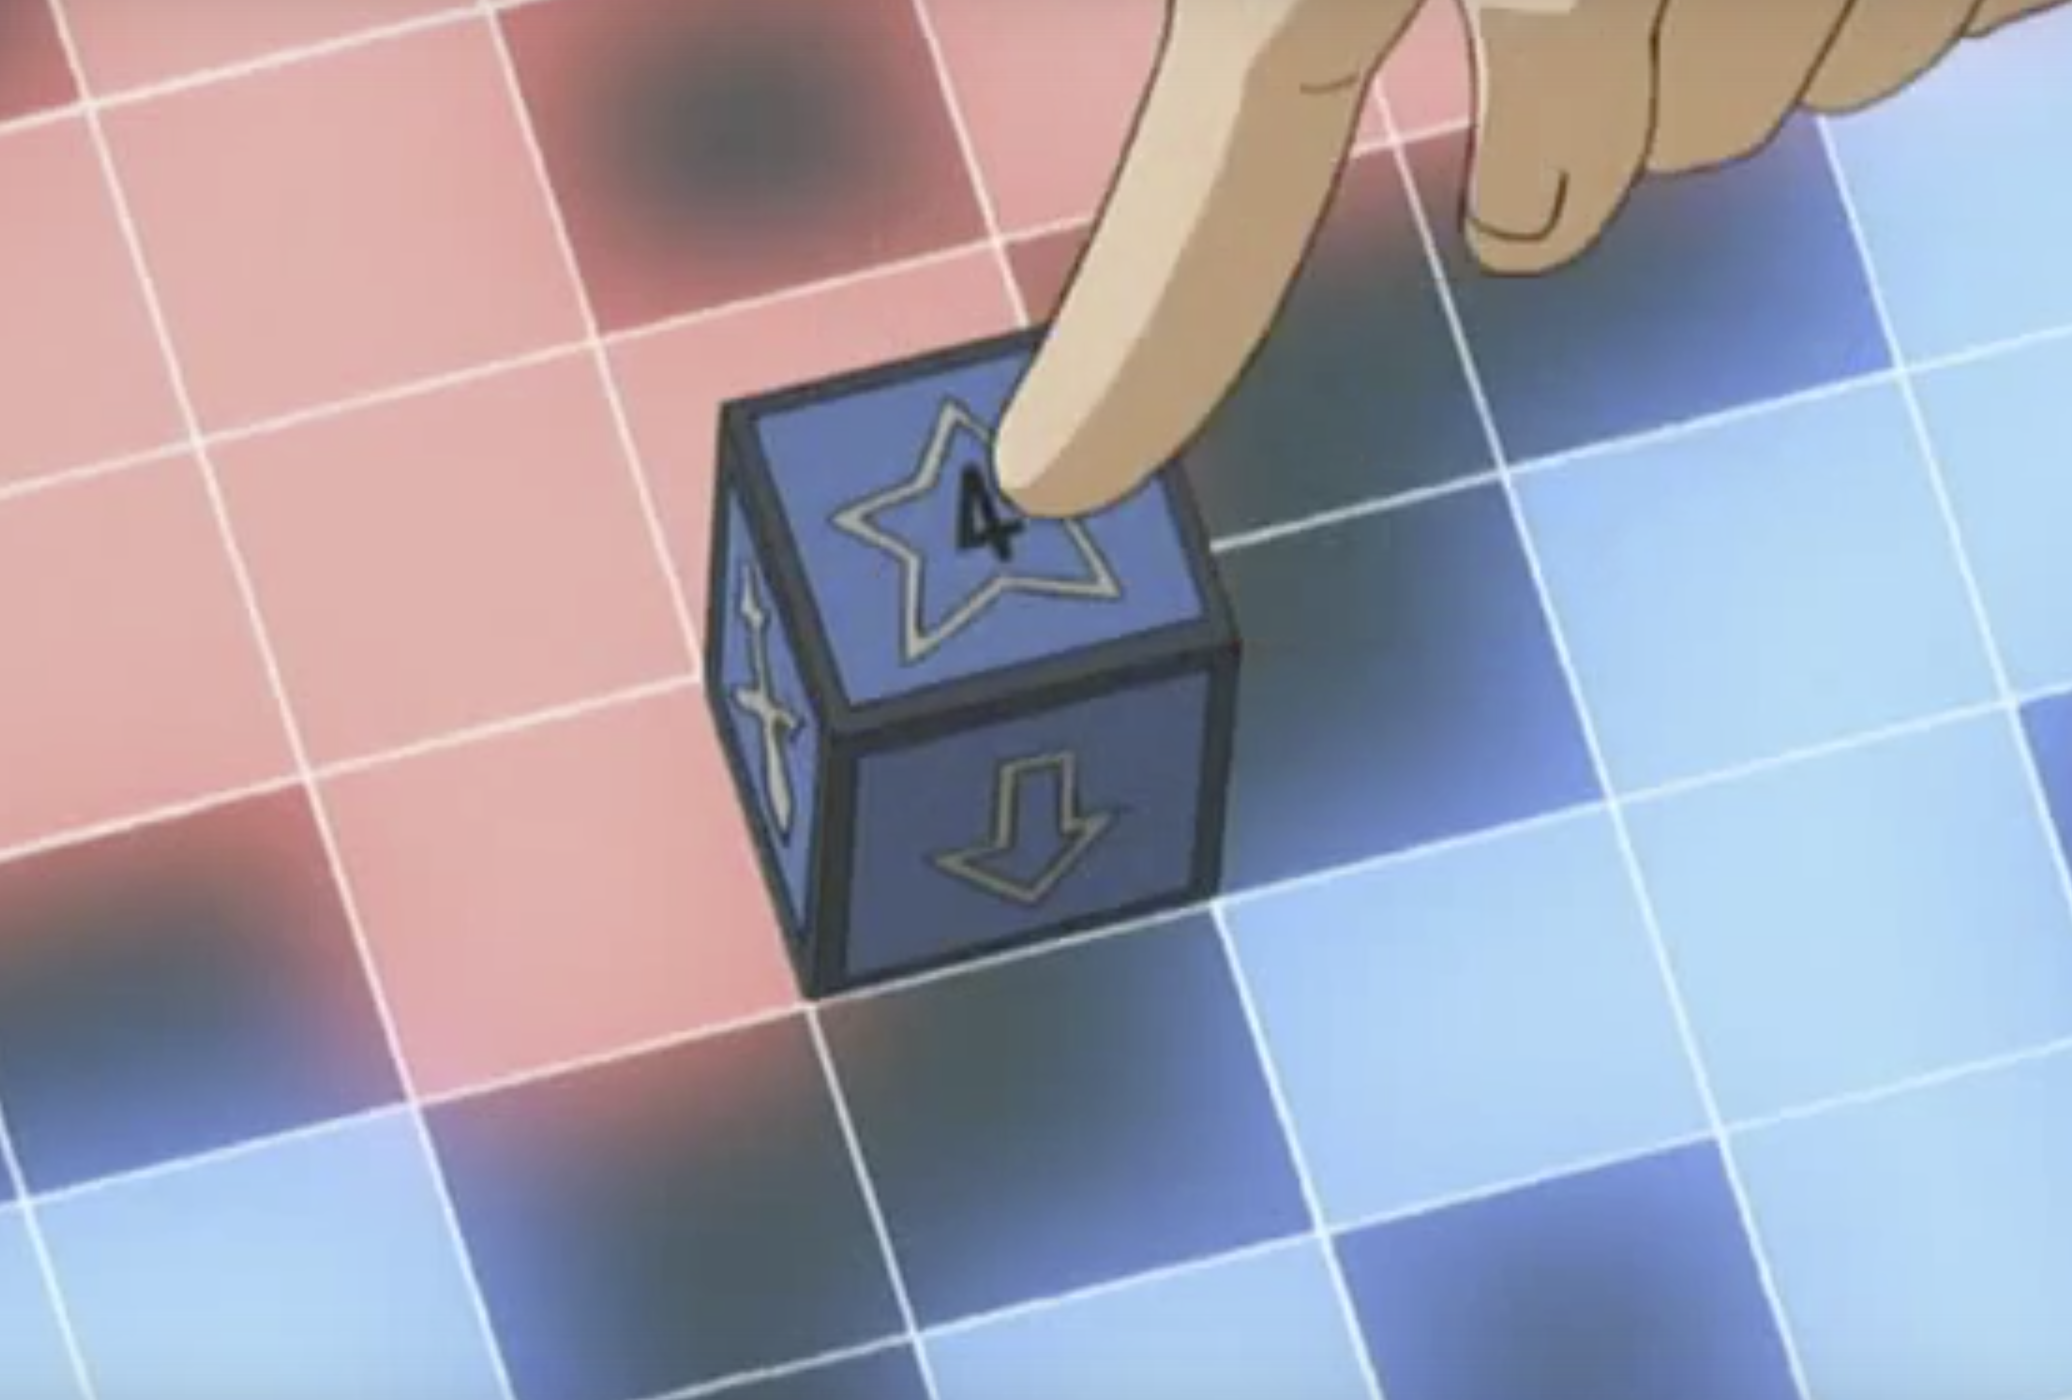
\includegraphics[width=0.75\textwidth]{YuGiTwo.png}
	\end{figure}

This provides an excellent analogy. Think of the history of music as the grid, and think of all the pieces of music ever created as the unfolded dice blocks. Then think of unfolding a dice onto the grid as composing a song. When this is done most beautifully (and also most impressively) is in the same situation which Yugi found himself in during this episode, \emph{place something down which fits perfectly into what surrounds it, but without overlapping with any of the currently existing pieces}. That is, pay attention to history and the playing field, and find what slots perfectly into the centre.

\subsection{Constraints and beauty}

\begin{center}
	\emph{When the constraints become the description of the beauty, true art has been achieved}
	\end{center}

The band Bell Witch have an incredibly beautiful song called Mirror Reaper. It is a soulful and mournful journey through the grief of two musicians who dedicate a portion of the song to their deceased close friend who was once also a member of the band. This song is incredibly slowly paced, with every next section coming as a necessity to that which preceeds it. It is noteworthy that this song is:
\begin{itemize}
	\item incredibly limited melodically,
	\item incredibly limited harmonically,
	\item incredibly limited rhythmically,
	\item incredibly limited instrumentally (only two musicians are needed to perform the entire thing),
	\item incredibly long, it runs for 83 minutes,
	\item is unmistakably ``metal",
	\item incredibly limited lyrically considering its length.
	\end{itemize}
At this point... what is left?? It is as though we have taken away every possible aspect of music that there is, yet the song is 83 minutes long! What does it even consist of in that case? Well, in my opinion, what remains are only the most difficult qualities to achieve in music composition:
\begin{itemize}
	\item atmosphere,
	\item mood,
	\item narrative,
	\item emotional communication,
	\item space,
	\item implication.
	\end{itemize}
If you listen to this song and you are bored for even a second, then you're not listening to it properly. The depth of the subtlety is indescribable. This is truly a remarkable piece of art, and the only way I could every explain why is by using the exact same sentences which I used to describe its limitations!! It's incredibly beautiful \emph{because} it is so melodically limited, and \emph{because} it is so harmonically limited, etc. I am forced to pay attention to the extreme details which are all there and moreover are incredibly impactful.

This to me, is the strongest link that there is between music and mathematics. Consider the fundamental theorem of abelian groups for example.

\begin{thm}[Fundamental Theorem of Abelian Groups]
	Let $A$ be an abelian group. Then there exists integers $r, k_1, \ldots, k_n \in \bb{N}$ with $k_i$ dividing $k_{i+1}$ for all $i = 1, \ldots, n-1$ as well as an isomorphism
	\begin{equation}
		A \cong \bb{Z}^r \oplus \bb{Z}_{k_1} \oplus \ldots \oplus \bb{Z}_{k_n}
		\end{equation}
	\end{thm}

Why is this Theorem beautiful? Because it makes abelian groups so unbelievably tangible. It tells you what Abelian groups \emph{are}. The theorem pertains to a mathematical object which is described with only four axioms! Pure mathematicians are sometimes critisized for having an appreciation for ``completely random" sets of axioms. This is simply not true though, pure mathematicians have an appreciation for completely random axioms \emph{which turn into something}.

This is identical to music and both parties can learn something from each other here. Mathematicians and musicians alike frequently fall into the trap of random experimentation. In my opinion it is not enough to technically speaking achieve a Theorem, nor to technically speaking create a piece of music, but instead one must achieve something like the Fundamental Theorem of Abelian Groups, or like Mirror Reaper, before something \emph{real} has been achieved.

\section{How to actually compose music}
\begin{center}
	\emph{What is a song?}
	\end{center}
Music played through a speaker does not sound the same as music played through headphones, however, this does not create hesitation when a song is to be identified. Played out-loud, through headphones, through car speakers, or even played live by physical instruments, one quickly latches onto the sense of familiarity when their favourite song plays.

A Mathematician might say “a song is identified up to natural equivalence”, as were the musician to play a wrong note at a non-crucial moment, it would be dramatic in that moment to suggest an entirely different song has been played.

Let us now draw a distinction between a song and an instance of a song. Emotionally, it feels as though this settles the dispute, an instance of a song is the familiar concept: a recording on a CD, a live performance, a cover, etc. However, the excited energy which pushes the concept of an “instance of a song” into clarity simultaneously pushes the concept of a “song” into abstraction. The song becomes a theoretical object, and an instance of a song a physical realisation of its platonic counterpart.

Other examples of pairings between theoretical objects and their physical counterparts are kindness paired with an act of kindness, an artistic experience paired with an artwork, or indeed the number five, paired with five rocks.

Where this becomes most interesting is in the mind of a composer. How does one compose when what they create is not what they are driven by? Explicitly, composer C does not create a song, but instead creates an instance of a song, so how ought C be driven?
The answer begins at a shift in perspective: one ought not forge a song, but instead one ought raise a song. Indeed, whether music is created or discovered is not known, but it is my contention that in either case the music should feel as though it was discovered. A good test is to see if it feels as though somebody else wrote it. Indeed, a creation born in a moment of true flow will be fascinating to that same craftsman at a later point.

Thus, to become a good composer is to become a good parent. A good parent patiently listens and follows their child’s interests without judgement nor concern for how that parent feels about the particular activity. In exactly the same way, a good composer does not write metal because metal is cool, but instead a good composer allows the song to find itself, through patient listening.
Where, in that case, does one begin when writing a song? The answer is that the process has already started, in fact it started long ago. Those who are compelled to compose have musical ideas already inside them, but they are covered in many layers of one’s own mind’s confusion and lack of self-awareness. Moreover, the musical idea is young, in fact, it is but an infant, so any ideas of its future are projected hopes from our own weak minds and thus must be ignored. Again, the job of the composer, is to be a good parent.

Obdurate begins with a blank score. A grand staff, piano. Excellent musical notation software must be chosen, the correct choice is Guitar Pro. A novelty amongst certain communities, but this program is cheap, efficient, intuitive, and the sounds are excellent.

First come chords, this by far is the most important part of the process. Beautiful chords have the power to generate emotion even when played in block pattern, with no sensible timing, on an overly digitalised piece of software. Never fall into the misbelief that having good quality sounds or instruments is crucial for good quality composition. The opening chords and oboe melody of A Metric Based on Insects has almost identical emotional pull when played on Guitar Pro as when played from the album (where the quality of the tones is higher).

Beyond this, is years of developing the skill of parenthood. Listening back to the block chords may call for attention to harmonic tempo, a rhythm, a melody, an extension, a retraction, a different tone, a layer, a sample, compression, equalisation, spoken word, invisible lyrics, etc. One follows one’s best judgement of decision. The song does not know of these concepts, it is the job of the composer to offer, in the same way that a child may not know of the concept of tennis, it is up to the parent to offer such a past time.

The most important part of the process is to enjoy the challenge of not knowing how to create the sound that you are after. As a concrete example, Comic Book Channel required guitar recordings (in fact, the entire album did in the end), and I do not play guitar. This is a hurdle and it is an opportunity. I simply learnt guitar and then recorded the tracks (in extremely small, bite sized chunks). The learning gained from this experience is indescribable. One inevitably comes across hurdles, one simply problem solves. The key is to keep making progress, the feeling of moving forward will help maintain motivation.

\subsection{Musical techniques}
\subsubsection{Harmonic tempo}
Harmonic tempos is the rate at which the harmony changes (for example, how rappidly chord changes occur). A lot of pop songs for examle will have the harmonic tempo in the chorus be double that of the verse. For instance, there may be a chord change once every two bars in the verse, and then a chord change every bar in the chorus.

How can we put an interesting spin on this though? What if we achieved variation in harmonic tempo whilst still maintaining the same number of chord changes per bar? Is this even possible?

Simple, we change the lengths of the bars! In the following excerpt (Comic Book Channel - Obdurate), the first section is in 5, and then the next in 3, but per bar the chord changes occur at the same rate.

(Comic Book Channel 2:50 - 4:23, 5:35 - 6:31).

\subsubsection{Personality}
\begin{center}
	\emph{We must avoid writing musician's music}.
	\end{center}
If you are a metal drummer, then it is likely that you enjoy playing as quickly and as loudly as possible, and with good reason! The level of intensity which a drum kit is capable of is an astonishing part of that instrument. However, metal drummers are very good examples of musicians who fall into the trap of writing ``musician's music", which essentially means music which can only be enjoyed by people who are also musicians of that same type. For instance, when I listen to particular drummers, I am left in awe over how intensely they play and for how long, but I don't \emph{feel} anything emotionally compelling from their composition. This is because the greatest appeal that the music has to be is the sensation of ``how on earth are they doing that"? Notice that this is a question which specifically pertains to the literal fact that this is a person playing a musical instrument. Compare this to the question ``how did they build such a strong universe?" Which pertains to ``more" than the literal performance of music via an instrument.

There are some songs which put you straight into that world right from the opening 0.1 seconds (literally). This is remarkable, and the technicalities of how this is done remains a mystery to me, however I know that it is the next concept which I will strive to master.

(A Metric Based on Insects opening minute). This is a relatively straight forward chord progression behind a relatively straight forward melody with certainly straight forward instrumentation. Yet this is a noteworthy moment, why? Because of the mournful universe it sets up right from the very onset. How could one attach a mathematical theory to this when the constituent components are so basic? There is ``more" to it than what the theory is capable of describing and thus we have achieved the aforementioned lift off from the constraints which define it.



\chapter{Story telling}
What are the foundational objects of mathematics? In fact this question is not as fruit baring as one would hope nor expect. Is the canonical answer ``sets"? Or ``types"? Or ``objects"? In any of these cases one must first present a \emph{story} before any insight can be drawn from these suggestions. My explicit claim is that these stories are part of mathematical objects themselves, and that mathematical foundations ought take this suggestion seriously. What this has to do with music will be made transparent in Section \ref{sec:mathematical_opera}.

\section{Depth}
\begin{center}
	\emph{What does it mean for something to be ``deep"?}
\end{center}
We can give a precise answer to this question, but we begin with an example. I claim that Chess is deep. When one first learns chess, they become aware of the basic rules, ie, the allowed and disallowed movements of the pieces. Once one is aware of the basic rules, one can study the basic chess principles:
\begin{itemize}
	\item Develop your pieces quickly.
	\item Control the center.
	\item Develop knights towards the center.
	\item Calculate forced moves first.
	\item Etc.
\end{itemize}
Then one can learn intermediate chess principles, this is the point where a greater level of ``depth" is achieved.
\begin{itemize}
	\item Develop a base knowledge of ``tournament openings".
	\item Learn critical pawn structures.
	\item Understand planning and development.
	\item Etc.
\end{itemize}
We notice the crucial point that only once the 0$^{\text{th}}$ layer of understanding has been achieved, can the 1$^{\text{st}}$ layer even make sense, let alone be understood.

After this come more advanced concepts.
\begin{itemize}
	\item Forks, skewers, pins.
	\item Tempos.
	\item Transitions.
	\item Sacrifices.
	\item Etc.
\end{itemize}
We notice again that this next layer can only be acheived once the previous has been.

There is still more. There is then threats, advanced end games, advanced patterns, different types of check mates and check mate threats, history, advanced calculation, etc.

The point, is that the \emph{minimum} amount of conceptual comprehension which is required in order to achieve understanding of some concepts which are genuinely relevant to the game is large. The fact that chess is capable of this is what makes Chess deep.

\begin{exercise}
	Write a formal definition of depth using the language of first order theories.
\end{exercise}

This concept of depth was revealed to me by studying mathematics and by talking to mathematicians.

Music composition is also deep. Some examples of basic compositional ideas are:
\begin{itemize}
	\item Basic chord progressions (block movement).
	\item Basic melody writing (avoid dramatic movement and respond to leaps with steps in the opposite direction).
	\item Basic rhythmic writing (tempo, beat, pulse, etc).
\end{itemize}

\section{More musical techniques}
Ultimatley one wants to develop their own musical techniques, and one must also keep in mind that rules were made to be broken. There is still value in opening up your mind by learning some of the creative general techniques people have developed in music writing.

\subsection{Melody (tension/release, steps)}
Consider one octave on a piano keyboard. Then there are 13 intervals (pairs of notes) we can create. They are unison, minor and major second, minor and major third, perfect fourth, tritone, perfect fifth, minor and major sixth, minor and major seventh, and octave. These are loosely categoriesed into three categories, consonant, dissonant, or context dependent. We have:

\begin{center}
	\begin{tabular}{| c | c | c |}
		\hline
		\textbf{Consonant} & \textbf{dissonant} & \textbf{context dependent}\\
		Unison & Minor/major second & Perfect fourth\\
		Minor/major third & tritone & \\
		Minor/major sixth & minor/major seventh\\
		Octave & & \\
		\hline
		\end{tabular}
	\end{center}

In general, people adore dissonance. It can be a source of tension. Consonance can be a source of release. There is also a concept of \emph{strong} and \emph{weak} points of a bar, and in the common practice period lots of tension was placed on the weak points of a bar, and lots of release moments at the strong parts of the bar.

An offering of creativity is that the perfect fourth is often classified as ``context dependent", in that it can sometimes be percieved as consonant and sometimes dissonant.

\begin{exercise}
	Create a piece of music where the perfect fourth is used both as a moment of tension, and as a moment of release.
	\end{exercise}

Dimitry Shostakovich has a beautiful piece of piano music called ``Fugue in A major" where \emph{only consonant intervals} are every used. This is a beautiful example of constraint writing and shows again how what is originally used as a description of the pieces limitations become the exact description of its beautiy.

\subsection{Layering}

Layering is a deeper concept, and it requires knowledge of more basic concepts in order to explain properly. A simple example of layering is \emph{harmonic layering}, where one instrument plays one chord, and another instrument plays a different chord over the top of that one, so that there are two harmonies being played simultaneously. Another simple example is melodic layering, where multiple melodies are played at once. A beautiful example of melodic layering is ``Escaping the Ruins" by Gareth Coker, this piece appears in the soundtrack to the video game ``Ori and the Blind Forest", 1:39 - 2:15.

Layering can be more abstract however. For instance, we spoke last time about harmonic tempo, where the rate at which chord changes occur is varied. One could layer even this. So that different instruments have different harmonic tempos. Another example is intesity layering, where different instruments play at different intensities. In the context of metal, incredibly quick drums, along with mid-tempo guitar, low tempo bass, and very low tempo vocals is very effective. An example of this is ``Shrines of Paralysis" by Ulcerate, 1:21 - 2:03.

Layering can be pushed so much further, and there is such thing as meta-layering, where layers are layered. Every musical technique can be layered. Last time I spoke about some more difficult to achieve musical elements/qualities; story telling, atmosphere, mood, space, implication, etc. These qualities are very difficult to achieve even only once, let alone multiple times and whilst well layered.
\begin{exercise}
	Write a piece with layered mood. One with layered space. One with layered implication, etc.
	\end{exercise}

\section{Mathematical opera}\label{sec:mathematical_opera}
What does mathematics have to learn from music?

Another anecdote: one time I was at band rehearsal and I was packing up my drum kit. I had three drums stacked up on top of each other, the floor tom, and then two rack toms sitting on top. My friendly vocalist wanted to help me move some of my drums to my car, and so he asked me what he could take. At this point in time, I had my hands full because I was holding my bass drum (which rendered me unable to point). I asked him to please take my floor tom and two rack toms, but he was not familiar with this terminology, and so asked me what I meant. I replied back ``the tower", and he looked at the three drums, and correctly picked up the ones I was hoping that he would.

What is interesting about this story, is that when I referred to the drums as what they \emph{were} (ie, a floor tom and two rack toms), he was confused and did not know what to do. However, when I referred to them as what they were \emph{not} (ie, a tower), he knew what I was referring to.

The point, is that \emph{it is sometimes more instructive to describe something as what it isn't than what it is}. A more sophisticated what to put this, is that sometimes it is sometimes more instructive to provide a \emph{narrative for navigation} than it is to provide an \emph{a precise definition}. Put simply: \emph{mathematics is meaningless when stripped of its narrative}.

This is why I believe so many mathematicians go through life perfectly fine without knowledge nor application of fundational concepts (eg, who many mathematicians can give the formal definition of an ordered sequence in the language of ZFC set theory, and of that percentage who can, how many think it matters?) The point is that narratives are so strong that one can make it astonishing far working off narratives alone without deep knowledge of the fundamental objects themselves. In fact, what even is an object? Does it matter? Why not take the brave step and say that objects \emph{do not exist} and instead only abstract relations exist. This would make narrative absolutely imperative, and I think that's where music comes in.

More specifically, opera. The stage has over centuries crafted the art of story telling using incredibly deep concepts such as metaphor, symbology, music, pace, masks, costume, etc. In fact, opera has become so good at describing narrative, that it is even capable of communicating incredibly complex and subtle aspects of being a human to enourmous audiences of diverce ages, cultures, and backgrounds. These aspects include and are not limitted to love, different shades of suffering, religion, different shades of fear and tranquility, family struggles, internal struggles, etc. So why not Cantor's theory of infinite sets? Or G\"{o}del's First Incompleteness Theorem?

\section{Some responses}
\emph{Stop trying to find your true self.} There are certainly drawbacks and limitations to a life philosophy which consists purely of the drive to find one's own ``true essence", especially in the abstract. This is certainly true. In the current context, we do \emph{not} suggest a search for one's ``true self" in any general context, but rather we suggest musing on one's true \emph{musical} self, and not souly so.

Let us rephrase the point. As deep and colourful as they are, let us consider one problematic point of subcultures. \emph{Self betrayal}. It happens all the time that people believe they have ``found themselves" in a subculture and then act in ways which they later regret. Tattoos, drugs, and crime provide great examples. This is an extreme point, but let's apply it to the special case of creating music. When one tries to create music of a particular style/or sound, one can fall into the trap of self betrayal, and suddenly success is identified with that which is accepted by the subculture. To put it simply, I just think this generates bad music. So authenticity has presented itself as necessary in my experience. This renders the concept of ``true self" as having application. This shifts the concept into \emph{applied philosophy}, and so I think is helpful. The main caution to be taken is the same as that with the more general approach, and that one risks making no movement. This can be overcome though and is reasonably easy to manage.

\emph{Music outside of creativity and exploration.} Essentially, this is just not where I see the depth and beauty in music, and so I ultimately do not have much to say on the topic. I believe that problems similar to the previous point have come out of viewing music in this way, and that bothers me, but I do myself well to remain mostly silent on this particular topic.

\emph{Creativity in repetition.} There is a tremendous amount which can be gained through mimicry. This is certainly true. However this should be seen as training and not as the final goal. There are tons of musical pieces I never released which sound identical to those pieces which inspired me. This is perfectly fine, but we live in a world where more musical releases are in incredibly small demand, so be humble, and release only which is worth existing.

\end{document}